% Chapter 2

\chapter{Foundations and Concepts} % Write in your own chapter title
\label{Chapter2}
\lhead{Chapter \ref{Chapter2}. 
\emph{Foundations and Concepts}} % Write in your own chapter title to set the page header

{\bf \small{
This chapter presents\dots
}}


\section{Introduction}
% what is machine learning
% machine learning is in the peak ot its popularity and we can find it everywhere

% the goal is to find the underlying function that explains some phenomenon, which would help us predict new events

% supervised vs unsupervised 

% linear regression is one typical example, often used in science

% two of the most popular families of ML methods are: kernel methods and neural networks

% kernel methods advantages, theory, convexity; disadvantes: scalability

% neural networks advantages: scalability, flexibility; disadvantages: lack of theory



\section{Kernels and Implicit Features}
% los kernels son centrales en ML
Kernels are central in \acrshort{ml}, and some of the most successful methods use them, such as \acrshort{svms} or \acrshort{gps}.
The main advantage of using kernels, as we will see, is that we can send our data to a high, even infinite, dimensional space, where the problems of interest, regression or classification, are expected to be easier. Moreover, this transformation is made implicitly by exploiting the reproducing property of the kernels. This is named the kernel trick, and we will explain more carefully later in this section.

% están relacionados con la VC dimension porque nos permiten  
By using kernels, we change our feature space, from a finite-dimensional one to a much larger one, with possibly infinite dimensions. Although this might ease the problem of learning a function that explains our data, we also can encounter some problems. One is the curse of dimensionality, that is, the cost of finding a solution to optimization problems typically scales super-linearly with the dimension of our data. Other problem is overfitting, when the data is placed in a high-dimensional space the hypothesis that can explain the data are more expressive, and if they fit too exactly to the training data, they could not generalize well to new data. However, as we will see later in this Chapter, these problems can be solved.


\subsection{Learning in Feature Spaces} %

\begin{figure}[t!]
    \centering
    \subfloat[][Simplified \fdata{iris} example.]{%    
    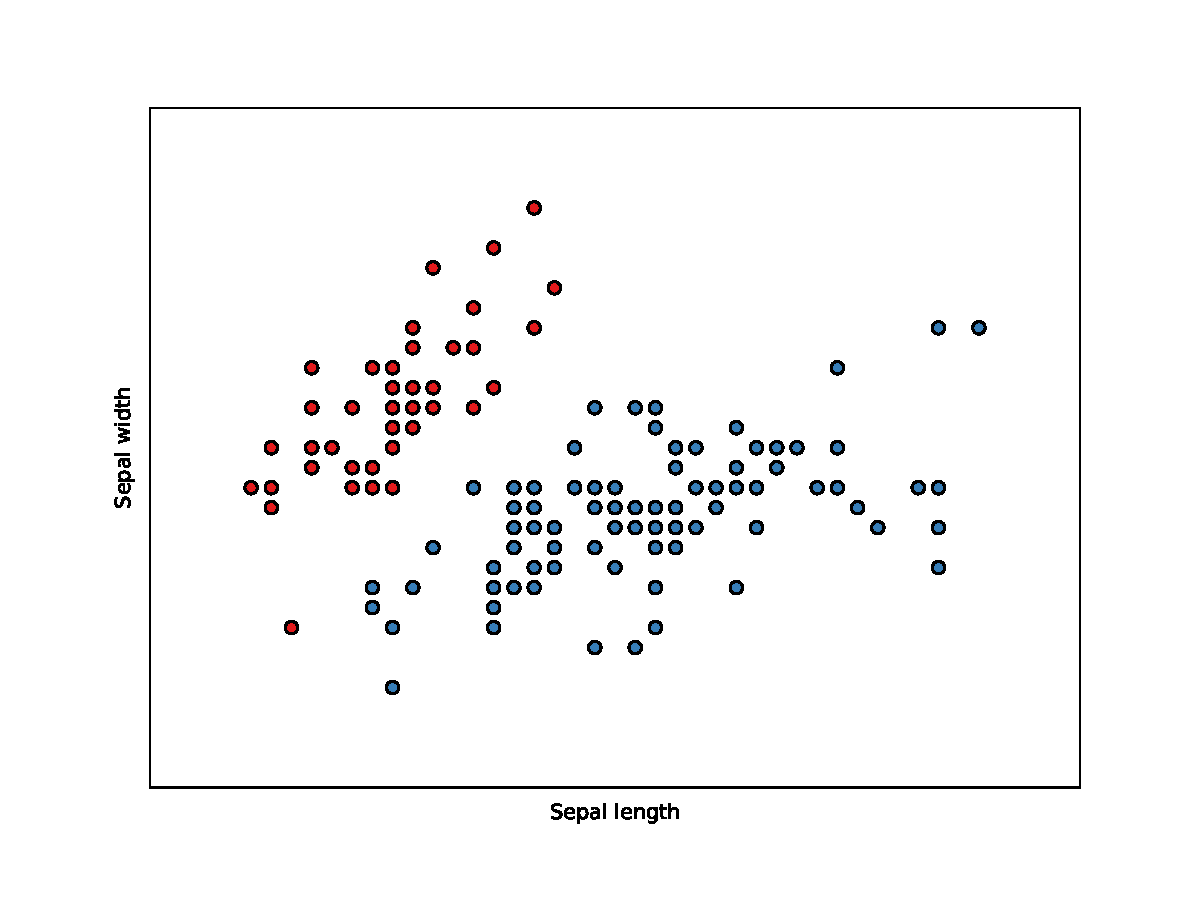
\includegraphics[width=0.45\textwidth]{Chapter2/Iris/iris.pdf}
    \label{fig:iris_example}}\quad%
    \subfloat[][Projections of simplified \fdata{iris} example.]{%
    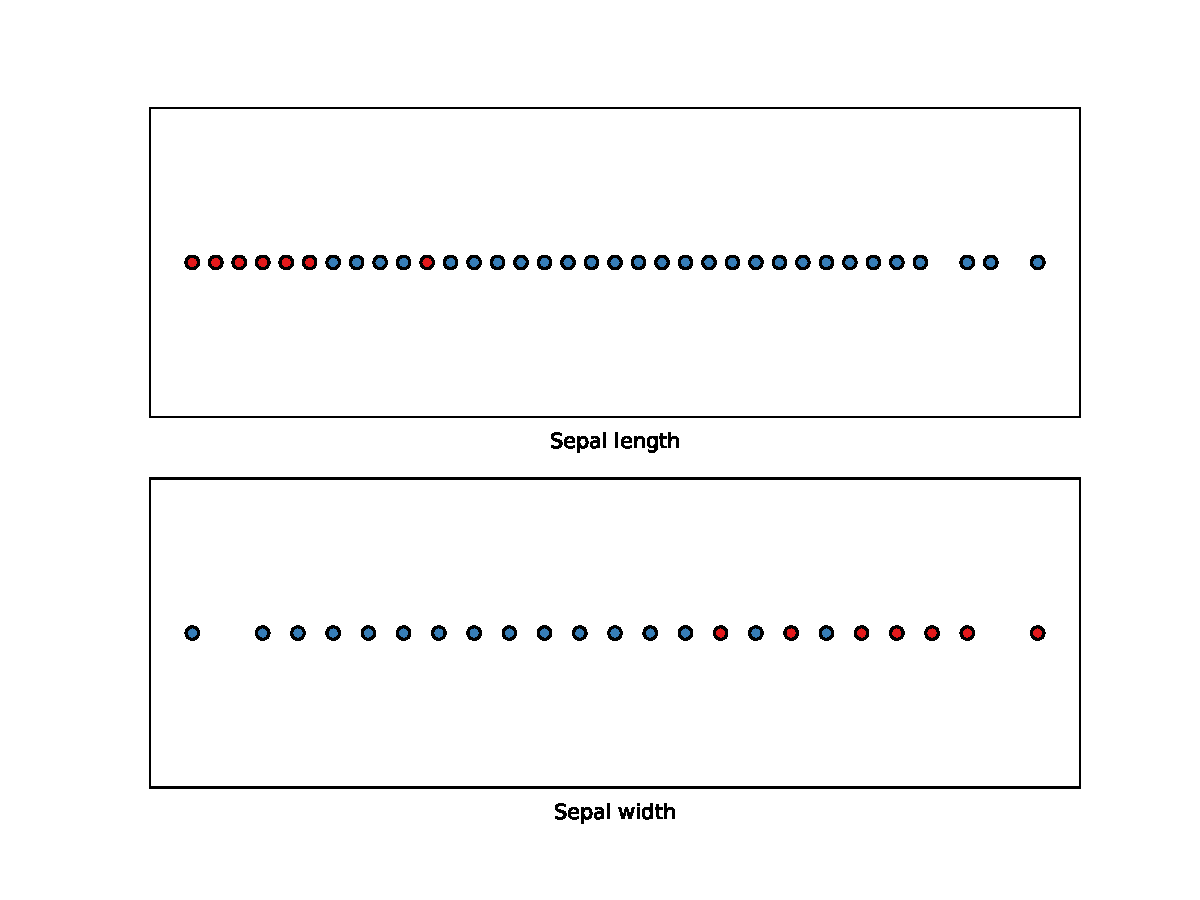
\includegraphics[width=0.45\textwidth]{Chapter2/Iris/projections_iris.pdf}
    \label{fig:iris_projections}}\\
    \caption{}
    \label{fig:iris}
\end{figure}

\begin{figure}[t!]
    \centering
    \subfloat[][Cubic regression problem. The underlying function, $f(x) = x^3$ is shown in orange, and the target values are the dots in blue.]{%    
    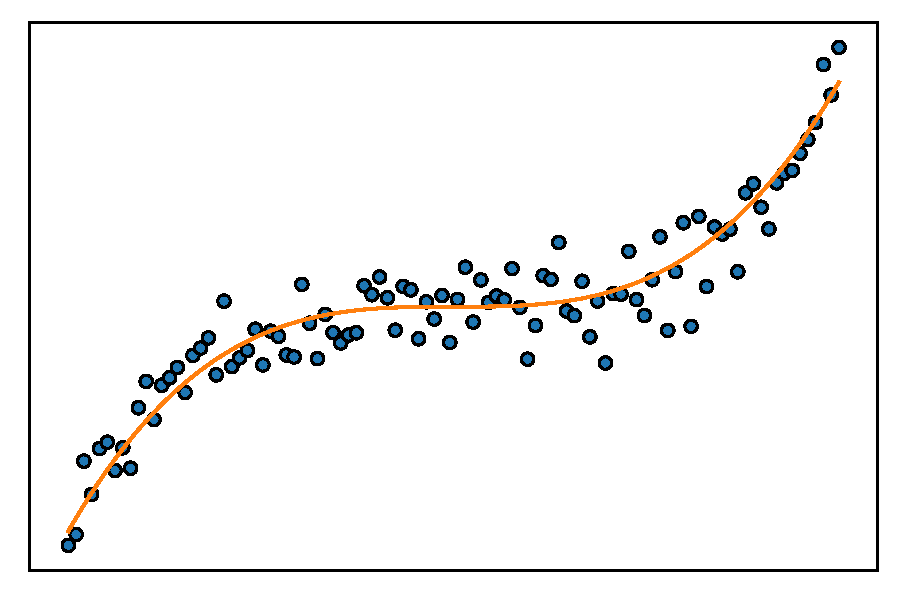
\includegraphics[width=0.3\textwidth]{Chapter2/CubicReg/regression_problem.pdf}
    \label{fig:cubicreg_example}}\quad%
    \subfloat[][Predictions with a linear feature space, including only $x$. The real function $f(x)=x^3$ is shown in orange and the predictions are the blue dots.]{%
    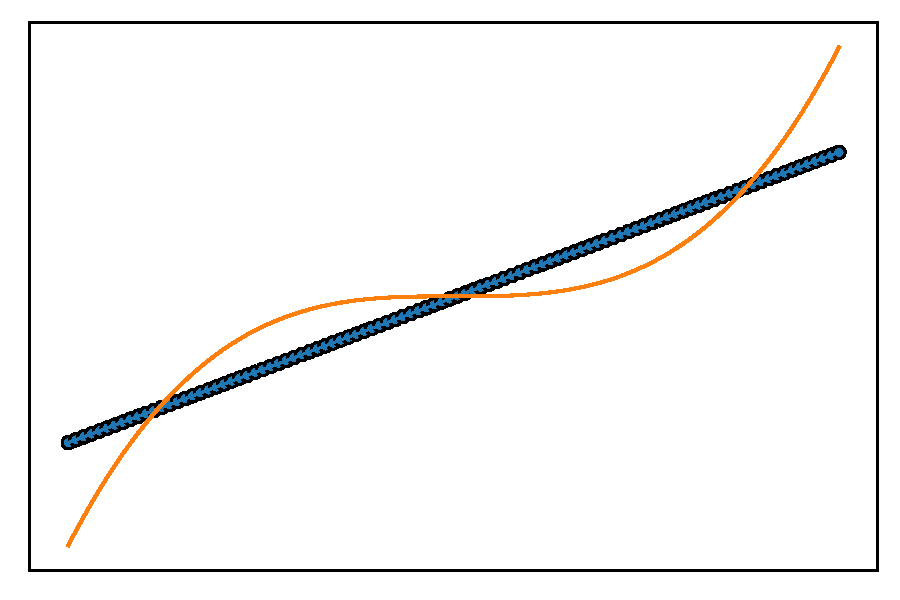
\includegraphics[width=0.3\textwidth]{Chapter2/CubicReg/regression_linearsol.pdf}
    \label{fig:cubicreg_linearsol}}\quad
    \subfloat[][Predictions with an extended feature space, including $x, x^2$ and $x^3$. The real function $f(x)=x^3$ is shown in orange and the predictions are the blue dots.]{%
    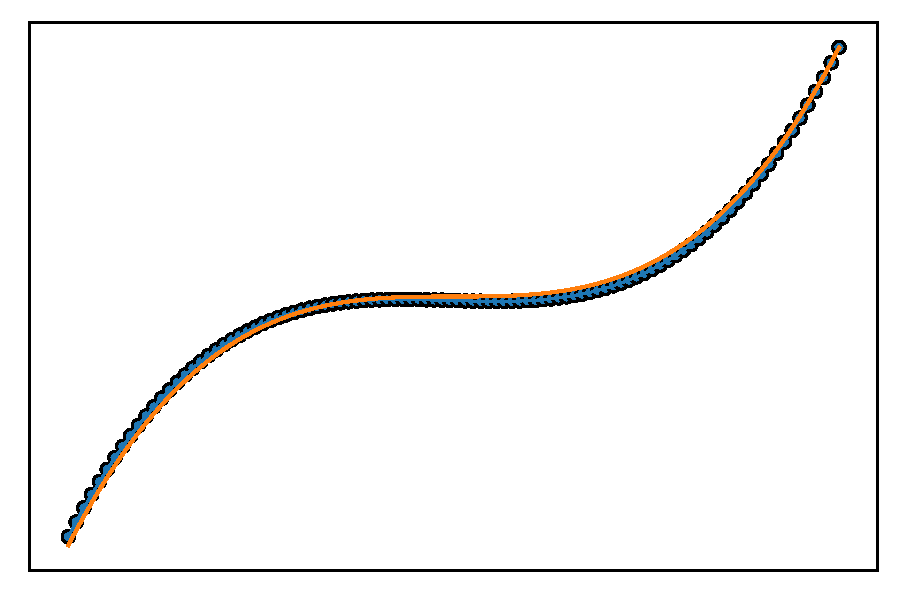
\includegraphics[width=0.3\textwidth]{Chapter2/CubicReg/regression_cubicsol.pdf}
    \label{fig:cubicreg_cubicsol}}
    \\
    \caption{}
    \label{fig:cubicreg}
\end{figure}

In \acrshort{ml} the choice of the feature space is crucial. If it is too small or too poor, it is not possible to find a good solution to our problem.
Consider the classification setting, when the feature space is low-dimensional, the classed are more overlapped and finding a decision boundary is more challenging. 
%
Take for example the popular \fdata{iris} dataset, where the goal is to discriminate between three species of iris flowers: \emph{setosa}, \emph{virginica} and \emph{versicolor}. To do this, $50$ samples from each species are gathered, and four features are measured for each sample: the length and width of the petals and of the sepals.
%
Now, for illustration purposes, we take a simplified version in which the goal is to discriminate the \emph{setosa} class from the rest, and where we consider only two features: the length and width of the sepals. In Figure~\ref{fig:iris_example} we represent the data corresponding to this simplified version of the \fdata{iris} problem, and we can observe that the two clouds of points are easily separable by a linear function. However, if, instead of the two-dimensional space, we consider just one feature, the problem is no longer separable. In Figure~\ref{fig:iris_projections} we note that the two classes are no longer separable.
%

For an example of how enlarging the feature space can lead to better solutions, consider a regression problem where we take $100$ one-dimensional points linearly distributed in the feature space, in this case $[-2, 2]$; then we compute the target values as $y_i = x_i^3 + \epsilon_i$, where $\epsilon_i \sim \normal{0, 1}$. This is a regression problem that we illustrate in Figure~\ref{fig:cubicreg_example}. If we consider a linear regression model with the original feature space, it will not be able to approximate well the function $f(x)=x^3$, and the solution is depicted in Figure~\ref{fig:cubicreg_linearsol}.
However, if we enlarge the feature space using the transformation $\phi(\cdot)$ defined as
\begin{equation}
    \begin{aligned}
        \nonumber
        \phi:\Xspace &\to\Xspace^3 \\
        x &\to (x, x^2, x^3) ,
    \end{aligned}
\end{equation}
then a linear regression model in this new space can find a good approximation, as the one shown in Figure~\ref{fig:cubicreg_cubicsol}.
%

This kind of result is one of the motivations for using kernels. 
As we will see later, the linear formulations, such as the Linear Regression or \acrshort{svms}, has a dual formulation, which does not depend directly on the features $x_i$, but on the inner products $\dotp{x_i}{x_j}$.
Consider now that we have the feature space $\Xspace = \reals^2$, and we consider the following function:
\begin{equation}
    \begin{aligned}
        \nonumber
        k: & &\reals^2 \times &\reals^2 & &\to& &\reals \\
        & &((x_1, x_2), & (y_1, y_2))   & &\to& ((x_1, x_2)^\intercal &(y_1, y_2) + c)^2 .
    \end{aligned}
\end{equation}
Now, we can observe the following fact:
\begin{equation}
    \nonumber
    \begin{aligned}
        &((x_1, x_2)^\intercal (y_1, y_2) + c)^2 \\
        &= \left(x_1 y_1 + x_2 y_2 + c \right)^2 \\
        &= x_1^2 y_1^2 + 2 x_1 y_1 x_2 y_1+ x_2^2 y_2^2 + 2 c x_1 y_1 + 2 c x_2 y_2 + c^2 \\
        &= \dotp{(c, \sqrt{2c} x_1, \sqrt{2c} x_2, \sqrt{2} x_1 x_2, x_1^2, x_2^2)}{(c, \sqrt{2c} y_1, \sqrt{2c} y_2, \sqrt{2} y_1 y_2, y_1^2, y_2^2)}.
        %&= \dotp{\psi((x_1, x_2))}{\psi((y_1, y_2))} .
    \end{aligned}
\end{equation}
Therefore, if we have a model that depends on the inner products of the data in our feature space $x, y \in \Xspace$, and we define these inner products as $k(x, y) = (x^\intercal y + c)^2$, we are implicitly enlarging the feature space with the transformation $\psi$, defined as
\begin{equation}
    \begin{aligned}
        \nonumber
        \psi: & &&\reals^2 & &\to& &\reals^6 \\
        & &(x_1,& x_2)& &\to& (c, \sqrt{2c} x_1, \sqrt{2c} x_2,& \sqrt{2} x_1 x_2, x_1^2, x_2^2) ,
    \end{aligned}
\end{equation}
such that $k(x, y) = \dotp{\psi(x)}{\psi(y)}$.
%
Here, the function $k(\cdot, \cdot)$ is a kernel function, in particular, this is the polynomial kernel, and $\psi(\cdot)$ is its associated feature transformation. 
We remark that in the dual formulation of linear models, which will be explained in detail later, all we need is to define a proper kernel function that must meet some requirements, and, as we will see, it has an associated feature transformation function; then, by defining the kernel function, we are implicitly enlarging our feature space.




% linear models use the original space
% low-dimensional data is more interpretable but less expresive: there exists feature selection techniques
% high-dimensional data is less interpretable but more expressive
% ejemplo de problema no lineal (cuadrático o cúbico de clasificación) no lineal y usar kernel polinómico
% esto es un kernel, y es útil porque podemos resolver los problemas más facilmente

\subsection{The Reproducing Kernel Map} % three characterizations
% rkhs
To make use of kernels and to ensure that they have a corresponding feature transformation function that extends our feature space, we have to define some concepts and give some previous results.
In first place, we define the inner product.
%
\begin{definition}[Inner Product]
    An inner product on vector space $\Vspace$ is a map
    $$\dotp{\cdot}{\cdot}: \Vspace \times \Vspace \to \reals , $$
    that for all $u, v, w \in \Vspace$ and $a, b \in \reals$ satisfy:
    \begin{enumerate}
        \item $\dotp{u}{a v + b w} = a\dotp{u}{v} + b\dotp{u}{w}$ (linear);
        \item $\dotp{u}{v} = \dotp{v}{u}$ (symmetric) ;
        \item $\dotp{u}{u} \geq 0, \; \dotp{u}{u} = 0 \implies u = 0$ (positive definite) .
    \end{enumerate} 
\end{definition}
%
Then, we define a positive definite kernel function, which has some similarities with the inner product.
\begin{definition}[Positive Definite Kernel]
    Given a non-empty set $\Xspace$, a symmetric function
    \begin{equation}
        \nonumber
        k: \Xspace \times \Xspace \to \reals
    \end{equation}
    is a positive definite kernel if for any set $x_1, \ldots, x_\nsamples \in \Xspace$ and $c_1, \ldots, c_\nsamples \in \reals$,
    \begin{equation}
        \nonumber
        \sum_{i=1}^\nsamples \sum_{j=1}^\nsamples c_i c_j k(x_i, x_j) \geq 0 ,
    \end{equation} 
    and if $\sum_{i=1}^\nsamples \sum_{j=1}^\nsamples c_i c_j k(x_i, x_j)$, then $c_1, \ldots, c_n = 0$.
\end{definition}
%
It can be seen that both the inner product and the kernel function are symmetric and positive-definite. The connection between both goes further, and we will see it below.
%
For simplicity, we will say positive kernel or just kernel instead of positive definite kernel. We can characterize a kernel also using finite sets and the corresponding matrices built using such kernel. To do this we need to define the Gram (or kernel) matrix and positive definite matrix first.
%
\begin{definition}[Gram Matrix]
    Given a symmetric function
    \begin{equation}
        \nonumber
        k: \Xspace \times \Xspace \to \reals
    \end{equation}
    and patterns $x_1, \ldots, x_\nsamples$, the matrix $\fm{K}$ with elements $\fm{K}_{ij} = k(x_i, x_j)$, with $i,j=1, \ldots, n$, is called the Gram matrix.
\end{definition}
%
\begin{definition}[Positive Definite Matrix]
    A matrix $K \in \reals^{n \times n}$ is positive definite if
    $\sum_{i=1}^n \sum_{i=1}^n K_{ij} c_i, c_j \geq 0$ 
    for any $c_1, \ldots, c_n \in \reals$ and if $\sum_{i=1}^n \sum_{i=1}^n K_{ij} c_i, c_j = 0$, then $c_1, \ldots, c_n = 0$.
\end{definition}
%
Then, it is easy to characterize a kernel function by its kernel matrices, as stated in the following lemma.
%
\begin{lemma}
    Given a non-empty set $\Xspace$, a symmetric function
    \begin{equation}
        \nonumber
        k: \Xspace \times \Xspace \to \reals
    \end{equation}
    is a positive definite kernel if for any set $x_1, \ldots, x_\nsamples \in \Xspace$ and $c_1, \ldots, c_\nsamples \in \reals$, the corresponding Gram matrix is positive definite.
\end{lemma}
%

As illustrated in the previous subsection, we are interested in using kernels to implicitly transform our data. Consider the map from $\Xspace$, a non-empty set, into the space of functions $f: \Xspace \to \reals$, which we denote as $\reals^\Xspace$, defined as 
    \begin{equation}
        \begin{aligned}
            \nonumber
            \phi: \Xspace &\to \reals^\Xspace \\
            x &\to k(\cdot, x) .
        \end{aligned}
    \end{equation}
Here, we are transforming each point $x$ into a function that assigns the value $\phi(\tilde{x}) = k(\tilde{x}, x)$ to every $\tilde{x} \in \Xspace$. That is, in the new space, $x$ is defined by its similarity, expressed by $k(\tilde{x}, x)$, to every other points $\tilde{x} \in \Xspace$. This transformation seems difficult to work with because our new features are functions.
However, we can define a feature space associated with $\phi$, with an inner product associated with the kernel function $k(\cdot, \cdot)$. To do this, we follow three steps: we Define a vector space from the image of $\phi$, define an inner product in such space, and show that this inner product satisfies $\dotp{\phi(\tilde{x})}{\phi(x)} = k(\tilde{x}, x)$.
We begin by considering all linear combinations of images of $\phi$, that is, the functions 
$$ f(\cdot) = \sum_{i=1}^n \alpha_i \phi(x_i) =\sum_{i=1}^n \alpha_i k(\cdot, x_i), $$
with $\alpha_1, \ldots, \alpha_n \in \reals$.
The set of such functions is a vector space $\Vspace_\phi \subset \reals^\Xspace$, since given other function 
$$ g(\cdot) = \sum_{i=1}^m \beta_i \phi(\tilde{x}_i) =\sum_{i=1}^n \beta_i k(\cdot, \tilde{x}_i) ,$$
with $\beta_1, \ldots, \beta_m \in \reals$,
we have that $f(\cdot) + g(\cdot) \in \Vspace_\phi$, and for any $a \in \reals$,  $a f(\cdot) \in \Vspace_\phi$.
Now, we can define an inner product in this vector space as 
$$ \dotp{f(\cdot)}{g(\cdot)} = \sum_{i=1}^n \sum_{i=1}^m \alpha_i \beta_j k(x_i, \tilde{x}_j),$$
and we have to check that it satisfies the properties of an inner product. It is easy to see its linearity, since it is a sum, and the symmetry property holds from the symmetry of the kernel function. Finally, to check that it is positive definite we observe that because $k(\cdot, \cdot)$ is positive definite,
$$ \dotp{f(\cdot)}{f(\cdot)} = \sum_{i=1}^n \sum_{j=1}^n \alpha_i \alpha_j k(x_i, x_j) \geq 0$$
for any $x_1, \ldots, x_n \in \Xspace$ and $\alpha_1, \ldots, \alpha_n \in \reals$, and if $\dotp{f(\cdot)}{f(\cdot)} = 0$, then $\alpha_1, \ldots, \alpha_n =0$, hence $f(\cdot) = 0$.
%
This inner product is defined for any pair of functions $f(\cdot), g(\cdot) \in \Vspace_\phi$, in particular, consider $g(\cdot) = \phi(\tilde{x}) = k(\cdot, \tilde{x})$, then, from the definitions, we have that
$$ \dotp{f}{k(\cdot, \tilde{x})} = \sum_{i=1}^n \alpha_i \phi(x_i) =\sum_{i=1}^n \alpha_i k(x_i, \tilde{x}) = f(\tilde{x}) .$$
That is, $k(\cdot, \tilde{x})$ is the representative of the evaluation on $\tilde{x}$. Moreover, we observe that with $f(x) = \phi(x)$,
$$ \dotp{\phi(x)}{\phi(\tilde{x})} = \dotp{k(\cdot, x)}{k(\cdot, \tilde{x})} = k(x, \tilde{x}) .$$  
This is the reproducing property of the kernel, and it defines an easy way of computing inner products in the feature space of functions $\reals^\Xspace$, to compute the inner product between $\phi(x)$ and $\phi(\tilde{x})$, we just need to compute the kernel value $k(x, \tilde{x})$.

\subsection{Reproducing Kernel Hilbert Spaces}
%
Kernels, with its reproducing property, have a close connection with a particular class of Hilbert spaces, which are named \acrfull{rkhss}. First, we give the definition of Hilbert space.
%
\begin{definition}[Hilbert Space]
    A Hilbert space is a vector space $\hilbertspace$ with an inner product $\dotp{\cdot}{\cdot}$, such that under the norm defined by $\norm{u} = \sqrt{\dotp{u}{u}}, \; u \in \hilbertspace$, it is a complete metric space.
\end{definition}
%
An example of Hilbert space is $\reals^d$ with the inner product defined as $\dotp{u}{v} = u^\intercal v$.
%
% The completeness of a space can be defined in terms of the convergence of its Cauchy sequences, but, for the goals of this work, we can omit the details. 
We are interested in drawing the connection between kernels and the \acrshort{rkhss}, which is given in the following definition.
\begin{definition}[\acrshort{rkhs}]
    Given a non-empty set $\Xspace$, a Hilbert space $\hilbertspace$ of functions $f: \Xspace \to \reals$ with an inner product $\dotp{\cdot}{\cdot}$ is an \acrshort{rkhs} if there exists a symmetric function $k: \Xspace \times \Xspace \to \reals$ such that $\dotp{f}{k(x, \cdot)} = f(x)$ for all $f \in \hilbertspace$, and $\overline{\Span{\set{k(\cdot, x), x \in \Xspace}}} = \hilbertspace$. 
\end{definition}
Here, $\Span{\set{k(\cdot, x), x \in \Xspace}}$ is the span of functions $k(\cdot, x)$, that is functions defined as
$$ f(\cdot) = \sum_{i=1}^n \alpha_i \phi(x_i) =\sum_{i=1}^n \alpha_i k(\cdot, x_i), $$
and $\overline{\mathcal{A}}$ is the completion of set $\mathcal{A}$, which include the set itself and the limits of all its Cauchy sequences.
Other way to characterize \acrshort{rkhss} is as the Hilbert spaces $\hilbertspace$ with continuous evaluation functionals, the maps
\begin{equation}
            \begin{aligned}
        \nonumber
        E_{x}: \hilbertspace &\to \reals \\
        f &\to f(x) .
    \end{aligned}
\end{equation}
In this case, according to the Riesz Theorem~\citep{Whittaker1991ACI}, for every $x \in \Xspace$ there exists a single $g_x \in \hilbertspace$ such that
$$ E_x(f) = \dotp{f}{g_x}, \; \forall f \in \hilbertspace.$$
In particular, for $f = g_{\tilde{x}}$ we have $E_x(g_{\tilde{x}}) = g_{{\tilde{x}}}(x) = \dotp{g_x}{g_{\tilde{x}}}$. If we define a function $k(x, \tilde{x}) = \dotp{g_x}{g_{\tilde{x}}}$, then we can see that it is a reproducing kernel. It is symmetric because of the symmetry of the inner product, and definite positive because the inner product is also positive definite. The reproducing property 
hold from the definitions if we consider $k(\cdot, x) = g_x$.
%
Observe that, given an \acrshort{rkhs}, a Hilbert space with continuous evaluation functionals, it defines a unique kernel that is the reproducing kernel for such space, where the uniqueness comes from the unique evaluation representatives in the Riesz Theorem.
%

It is also possible to prove the converse, that is, given a positive definite kernel function, there exists an associated \acrshort{rkhs}.
To do that we need to generate a Hilbert space from a kernel function, which is done by considering its associated integral operator, whose properties are expressed in the Mercer theorem. In this theorem we use some concepts of measure theory. 
%
Given a non-empty set $\Xspace$, we consider a measurable space $(\Xspace, \mu)$ where $\mu$ is the measure. The expression ``almost everywhere'' means in every subset $\mathcal{S} \subset \Xspace$ such that $\mu(\mathcal{S}) \neq 0$. We also use the formulation $L_2(\Xspace)$ for the functions $f: \Xspace \to \reals$ that are measurable, that is,
$$ \int_{\Xspace} f(x) d\mu(x) < \infty .$$

\begin{definition}[Mercer Kernel]
    Let $k: \Xspace \times \Xspace \to \reals$ a symmetric continuous function, such that the integral operator 
    \begin{equation}
        \begin{aligned}
    \nonumber
    T_k: L_2(\Xspace) &\to L_2(\Xspace) \\
    f &\to \int_\Xspace k(x, \tilde{x}) f(x) d \mu(\tilde{x}) 
\end{aligned}
\end{equation}    
is positive definite; that is; for any $f \in L_2(\Xspace)$, 
\begin{equation}
    \nonumber
    \int_{\Xspace \times \Xspace} k(x, \tilde{x}) f(x) f(\tilde{x}) d\mu(x) d\mu(\tilde{x}) \geq 0 ,
\end{equation}
then $k$ is a Mercer kernel
\end{definition}

\begin{theorem}[Mercer Theorem]    
Let $k$ be a Mercer kernel and consider the normalized eigenfunctions $\psi_i \in L_s(\Xspace)$ and associated eigenvalues $\lambda_i$ of the operator $T_k$, such that
$$ T_k(\psi_i) = \lambda_i \psi_i , $$
then $\lambda_i > 0$ and $k(x, \tilde{x}) = \sum_{i=1}^\infty \lambda_i \psi_i(x) \psi_i(\tilde{x})$ almost everywhere, where the eigenvalues $\lambda_i$ are sorted in non-increasing order. 
\end{theorem}
%
With this result, we can construct a Hilbert space whose reproducing kernel is $k$.
Consider the following feature transformation
\begin{equation}
    \begin{aligned}
        \nonumber
        \phi: \Xspace &\to l_2 \\
        x &\to \left(\sqrt{\lambda_1} \psi_1(x), \sqrt{\lambda_2} \psi_2(x), \ldots \right) ,
    \end{aligned}
\end{equation}
where $l_2$ is the space of all sequences $(x_n)_{n \in \naturals}$ such that $$ \sum_{n \in \naturals} x_n < \infty .$$
In this space, the inner product between $\phi(x)$ and $\phi(\tilde{x})$ is defined as
$$ \dotp{\phi(x)}{\phi(\tilde{x})} = \sum_{i=1}^\infty \lambda_i \psi_i(x) \psi_i(\tilde{x}),$$ which, by the Mercer theorem, is equivalent to saying that $\dotp{\phi(x)}{\phi(\tilde{x})} = k(x, \tilde{x})$.

Then, we have seen that there is a one-to-one correspondence between positive definite kernels and \acrshort{rkhss}. Given an \acrshort{rkhs} there is a single kernel function that has the reproducing property in that space. Also, given a positive definite kernel $k$, there exists an associated \acrshort{rkhs} such that $k$ is its reproducing kernel. 

% mercer theorem?

% kernels as a measure of distance
% ejemplo de kernel Gaussiano e implicit transformation









\section{Risk and Regularization}
To automatize the learning process, which is the goal of \acrshort{ml}, it is necessary to define a criterion to measure the performance of the functions $f: \Xspace \to \Yspace$ estimated from the data.
At each particular sample $(x_i, y_i)$ we can give a metric of how close we are to our desired goal, this is the selected loss function. If we have a classification problem, we may want to minimize the number of incorrectly classified patterns, but this quantity is not differentiable and not easy to work with. In regression problems, we would like to minimize the distance between the regression function and the training target values, but there are also multiple ways to define this distance. 
%

Anyway, independently of the chosen loss function, the data that we use have been sampled, and we do not know the distribution. There are some samples more important than others, because they belong to an area of high probability, according to this unknown distribution. Getting a bad result, as defined by the loss function, in a sample that is an outlier of the distribution is not that relevant, because few data is expected to be sampled in its neighborhood. 
To account for this, we define the expected risk, which we want to minimize. Nevertheless, since the distribution is unknown, we consider it in an implicit way by minimizing the empirical risk.

%
However, when minimizing the empirical risk instead of the expected one, we might find that we are too influenced by the particular sample that we have been given.  If the training data is too scarce, or also if we have some prior knowledge that we want to incorporate to the learning process, the regularization of the models can be helpful, as we will describe.
%
Moreover, when we use linear models to minimize his regularized risk, there is a result that describes the solution in terms of the training data, which is crucial for kernel methods, especially where the linear model is built in an infinite dimensional space.

\subsection{Loss Functions}
Given a feature space $\Xspace$ and a target space $\Yspace$, the criterion that we use to measure the performance of our estimates $f: \Xspace \to \Yspace$ is defined by the loss functions.
Here, we give the definition of loss function and present the losses that we will use in the rest of this work.

\begin{definition}[Loss Function]
    Denote $(y, f(x))$ as the pairs consisting on an observation $y \in \Yspace$ and a prediction $f(x) \in \Yspace$, with $x \in \Xspace$ an element of the feature space, then any map
    \begin{equation}
        \begin{aligned}
    \nonumber
    \lossf: &\Yspace \times \Yspace &\to &&[0, \infty) \\
    &(y, f(x)) &\to  && \lossf(y, f(x)) 
\end{aligned}
\end{equation}
  %  $$ \lossf: \Yspace \times \Yspace \to [0, \infty)$$    
    such that $\lossf(y, y) = 0$ for all $y \in \Yspace$ is a loss function.
\end{definition}
Observe that $\lossf(\cdot, \cdot)$ is a non-negative function and the perfect prediction always achieves its minimum value.

% Classification
In the binary classification problems, if we want to minimize the number of misclassified patterns, we use the \emph{accuracy} loss, which is defined as
\begin{equation}
    \nonumber
    \lossf(y, f(x)) = 
    \begin{cases}
        0, & y = f(x) ,\\
        1, & y \neq f(x) .
    \end{cases}
\end{equation}
However, this function only takes into account if the example is correctly classified or not, but we might also want to take into account the confidence that we have in this decision. If we use the labels $\set{-1, 1}$ to denote the two classes, then we can look at the number $y f(x)$ to check if the decision is correct, only if $y f(x) > 0$ the pattern is correctly classified. That is, we are looking at a single value to determine the success of our decision, and we can also use it to define a confidence. For example, we can consider that in those patterns where $0 < y f(x) < 1$, although correctly classified, the confidence that we have to make such decision is not enough, and only when $y f(x) \geq 1$ we consider that it is a correct classification. We can interpret this as a confidence margin, and the loss function that implements this is called \emph{soft margin}, or also \emph{hinge} loss, which is defined as
\begin{equation}
    \label{eq:hinge_def}
    \lossf(y, f(x)) = 
    \begin{cases}
        0, & y f(x) \geq 1 ,\\
        1 - y f(x), & y f(x) < 1 .
    \end{cases}
\end{equation}
This is a continuous function where we can observe two charactistics. One is confidence margin where we ask $y f(x) \geq 1$ to consider it a decision without penalization. The other, is that the penalization grows linearly as $y f(x)$ decreases.
%
A modification of the hinge loss considers the same margin, but the penalization for the misclassified patterns grows as a quadratic function. This is the \emph{squared hinge} loss, whose expression is
\begin{equation}
    \label{eq:sqhinge_def}
    \lossf(y, f(x)) = 
    \begin{cases}
        0, & y f(x) \geq 1 ,\\
        (1 - y f(x))^2, & y f(x) < 1 .
    \end{cases}
\end{equation}
%
Finally, another commonly used function is the \emph{logistic loss}, where the classes are labeled as $\set{0, 1}$. With this loss, we model $P(y=1 \vert x)$, that is, the probability of $x$ being a pattern from class $1$, by using the sigmoid function $s(\cdot)$ as 
$$ s(f(x)) = \frac{1}{1 + \exp{(-f(x))}} .$$
Here, although $f(x) \in \reals$, $s(f(x)) \in (0, 1)$, so we can see it as the probability of being from class $1$. Then, the loss function is defined as 
\begin{equation}
    \label{eq:logistic_def}
    \lossf(y, f(x)) = - y \log{(s(f(x)))} - (1 - y) \log{(1 - s(f(x)))} .
\end{equation} 
Here, given for example a pattern from class $y=1$, only the first term is active, and the larger $f(x)$ is, the closer $s(f(x))$ gets to $1$, so the penalization is smaller.
In the binary classification scenario, the \emph{logistic} loss resembles the \emph{hinge} one. 

The formulae~\eqref{eq:logistic_def} also looks like the definition of entropy, so it is also named \emph{cross-entropy} loss. 
With the entropy interpretation, this loss is easily adaptable to the multi-class case with classes $\set{1, \ldots, C}$. Consider the one-hot encoding vector $\fv{y}$ of length $C$, such that $\fv{y}_c = 1$ if $y=c$ and $\fv{y}_c = 0$ otherwise, for $c=1, \ldots, C$.
Now, we can model the probabilities $P(y=c \vert x) = f_c(x)$ with $c \in \set{1, \ldots, C}$ and form the corresponding vector $\fv{f}(x)$; then, the multi-class \emph{cross-entropy} loss is defined as 
\begin{equation}
    \label{eq:crossentropy_def}
    \lossf(\fv{y}, f(x)) = - \sum_{c=1}^C \fv{y}_i \log{(s(\fv{f}_i(x)))} .
\end{equation} 
For the rest of loss functions there are also proposals for extending them to the multi-class case, but we will not use them in this work.

%Regression
In the regression problems, given a pair $(x, y) \in \Xspace \times \Yspace$, the goal is to minimize the distance between the observed target $y$ and our prediction $f(x)$; then, a natural loss is the \emph{absolute} loss function, defined as 
\begin{equation}
    \label{eq:abs_def}
    \lossf(y, f(x)) = \abs{y - f(x)}.
\end{equation}
Here, any mistake is penalized, but there might be some cases when the targets are noisy, so we would like to have some room for small errors. Concretely, if $f(\cdot)$ is the perfect regression function, the target values might be $y = f(x) + z$ with $z \sim \normal{0, \sigma}$; then, it might be not sensible to not penalize those errors that can be explained by this noise. This is done in the \emph{$\epsilon$-insensitive} loss function, which is expressed as 
\begin{equation}
    \label{eq:epsins_def}
    \lossf(y, f(x)) = 
    \begin{cases}
        0, & \abs{y - f(x)} \leq \epsilon ,\\
        \abs{y - f(x)} - \epsilon, & \abs{y - f(x)} > \epsilon .\\
    \end{cases}
\end{equation} 
Here, $\epsilon$ is a hyperparameter and have to be selected for each specific problem. Also, observe that with $\epsilon =0$, we have the \emph{absolute} loss.
%
The regression losses presented are based on the absolute value $\abs{y - f(x)}$, thus, they are not differentiable. One alternative is to use the squared value of the distance, as expressed in the \emph{squared} loss:
\begin{equation}
    \label{eq:sq_def}
    \lossf(y, f(x)) = (y - f(x))^2.
\end{equation}
% and, analogously, the \emph{squared $\epsilon$-insensitive} loss, defined as
% \begin{equation}
%     \label{eq:epsins_def}
%     \lossf(y, f(x)) = 
%     \begin{cases}
%         0, & \abs{y - f(x)} \leq \epsilon ,\\
%         \abs{y - f(x)} - \epsilon, & \abs{y - f(x)} > \epsilon .\\
%     \end{cases}
% \end{equation} 
The \emph{squared} loss is also easily adaptable to the multi-target regression problems. Consider the case with $K$ targets for each feature vector $x$, that is, $\fv{y}$ are vectors of length $K$, and we produce the corresponding vector of predictions $\fv{f}(x)$; then, the multi-target \emph{squared} loss is
\begin{equation}
    \label{eq:sqmulti_def}
    \lossf(y, f(x)) =  \norm{\fv{y} - \fv{f}(x)}^2.
\end{equation}


\subsection{Empirical and Expected Risk} 
In \acrshort{ml}, we have a feature space $\Xspace$ and a target (or label) space $\Yspace$, and we believe that there is a function $f: \Xspace \to \Yspace$, and if we have a good estimate of such function, we will be able to predict new target values $y$ given a pattern $x$. Take for example the popular problem \fdata{MNIST} of handwritten digits, where the feature space $\Xspace$ is the space of $28 \times 28$ matrices with values in $[0, 1]$, corresponding to the pixels of $28 \times 28$ grayscale images.
Once we have selected the most adequate loss functions for our goal, we have to minimize the loss function 
%

\subsection{Regularized Risk Functional}
% conexión con el repr. theorem


\subsection{Representer Theorem} % 
% aunque sea una transformación implicita, tenemos el Rep. Th. para ayudarnos

% este resultado está relacionado con la dualidad de los problemas lineales, que veremos más adelante
















\section{Learning Theory}
% Introducción de Vapnik?
% 
%

% regression problem: the most simple example is linear regression, used in many sciences


% classification problem: logistic regression

% joint formulation for both 


\subsection{Uniform Convergence and Consistency}
\subsection{VC dimension and Structural Learning}


\subsection{Maximum Margin Hyperplane}
% otra forma de limitar la capacidad es considerar solo las hipótesis que maximizan la distancia entre las clases

% teorema de Vapnik

% esta idea constituye la base de las SVM





\section{Optimization}
\subsection{Convex Optimization}
\subsection{Unconstrained Problems}
\subsection{Constrained Problems}


\section{Support Vector Machines}
\subsection{Linearly Separable Case}
\subsection{Non-Linearly Separable Case}
\subsection{Kernel Extension}
\subsection{SVM properties}
%\subsection{Connection with Structural Learning}
\subsection{SVM Variants}

\section{Conclusions}\label{sec-conclusions-1}

In this chapter, we covered\dots
